% Autor: Milan Vrbas <xvrbas01>

\documentclass[a4paper, 12pt]{article} % definice třídy dokumentu a nastavení vlastností

% Packages
\usepackage[utf8]{inputenc} % nastavení kódování
\usepackage{graphicx} % obrázky
\usepackage{times} % font
\usepackage[czech]{babel} % čeština
\usepackage[T1]{fontenc} % nastavení kódování fontů
\usepackage[left=2cm, text={17cm, 24cm}, top=3cm]{geometry} % nastavení rozměrů stránky
\usepackage[unicode]{hyperref} % odkazy
\usepackage{fancyhdr} % zkrášlení stránky

\pagestyle{fancy}
\fancyhf{}
\fancyfoot[C]{\thepage} % čára na začátku stránky

\begin{document}
\begin{titlepage}
    \begin{center}
        \scalebox{0.15}{
\includegraphics{pictures/FIT_logo.png}} \\
        \vspace{\stretch{0.382}}
        \Huge{Návrh projektu} \\
        \Large{\textbf{Organizátor táborových bodů }} \\
        \large{ITU – Tvorba uživatelských rozhrání }
        \vspace{\stretch{0.618}}
    \end{center}

    {\large \today \hfill
        \large
        \begin{tabular}{l l}
        \textbf{Milan Vrbas} & \quad \textbf{xvrbas01}\\
        Jan Juračka           & \quad xjurac07      \\
        \end{tabular}
        }
\end{titlepage}

\tableofcontents
\thispagestyle{empty}
\newpage

\section{Zadání}
\subsection{Uživatelský průzkum a specifikace}
Naše webová aplikace je určena pro táborové vedoucí Líseckého tábora. Umožňuje jim jednoduše 
sledovat týmové výsledky, zadávat body za různé soutěže a hry, a vyhlašovat denní i celkové 
vítěze. Cílem aplikace je zefektivnit organizaci bodování, eliminovat nutnost ručních zápisů 
a výpočtů a poskytnout přehledné, snadno dostupné zobrazení výsledků prostřednictvím 
intuitivního webového rozhraní. \\
V rámci projektu jsme provedli rozhovory s jednotlivými táborovými vedoucími z našeho okruhu, 
abychom ověřili, zda náš návrh odpovídá jejich potřebám, je uživatelsky srozumitelný a 
obsahuje všechny klíčové funkce.

\subsubsection{Rozhovor 1. člena týmu s uživatelem}
\begin{itemize}
    \item \textbf{Otázka č.1: Jak hodnotíte jednoduchost a přehlednost aplikace?} \\
    Odpověď: \textit{Aplikace mi přijde příjemně jednoduchá. Dělá přesně to, co potřebuji, 
    a líbí se mi, že není přehlcená funkcemi, které bych nevyužil. Je tak akorát zaměřená na 
    jeden hlavní úkol, což oceňuji.}

    \item \textbf{Otázka č.2: Jak se vám líbí uspořádání tabulky a její funkčnost?} \\
    Odpověď: \textit{Líbí se mi uspořádání do jedné tabulky, kde jsou body přehledně zobrazeny. 
    Vše je srozumitelné, takže mohu rychle zjistit výsledky, které potřebuji.}

    \item \textbf{Otázka č.3: Co si myslíte o použitém designu a ikonách v aplikaci?} \\
    Odpověď: \textit{Celkově je design jednoduchý a dobře odpovídá jednoduchosti aplikace. 
    Jen mi přijdou některé ikony trochu neintuitivní. Mohlo by být užitečné přidat ke každé 
    ikoně krátký popisek nebo tooltip, aby bylo hned jasné, co znamenají nebo případně pozměnit 
    ikonu samotnou.}

    \item \textbf{Otázka č.4: Pochopil jste zcela funkci pro zadávání týmových a herních bodů?} \\
    Odpověď: \textit{Při tvorbě týmů chápu, jak fungují herní a celkové body, ale myslím, že 
    by se to dalo ještě trochu vylepšit, aby to bylo úplně jasné a intuitivní. Možná by bylo 
    dobré mít možnost přizpůsobit zobrazení nebo doplnit další vysvětlení.}

    \item \textbf{Otázka č.5: Jak vnímáte celkový vzhled a pocit z aplikace?} \\
    Odpověď: \textit{Celkově se mi aplikace líbí a mám pocit, že dobře zapadá do toho, jak by 
    měla fungovat. Těším se, až ji budu moci vyzkoušet v praxi. Určitě bude skvělé mít vše 
    pohromadě a nemuset se starat o složité papírové bodování.}

    \item \textbf{Otázka č.6: Napadá vás něco, co by aplikaci vylepšilo?} \\
    Odpověď: \textit{Možná by bylo fajn mít možnost přidat ke každé hře pár poznámek nebo 
    komentářů, co se během hry stalo, abychom si to mohli později připomenout.}

    \item \textbf{Otázka č.7: Považujete aplikaci za vhodnou pro týmové využití?} \\
    Odpověď: \textit{Ano, myslím, že bude dobře použitelná i pro více vedoucích. Pokud bude 
    sdílení výsledků mezi vedoucími jednoduché a rychlé, určitě se mezi námi osvědčí.}

    \item \textbf{Otázka č.8: Vidíte potenciál aplikace pro širší využití i mimo jeden 
    konkrétní tábor?} \\
    Odpověď: \textit{Rozhodně. I když je aplikace navržena pro náš tábor, myslím, že by se 
    mohla časem přizpůsobit, aby fungovala univerzálně pro různé tábory. Současná verze nám 
    ale bohatě stačí a splňuje naše požadavky.}

\end{itemize}

\subsubsection{Rozhovor 2. člena týmu s uživatelem}
\begin{itemize}
    \item \textbf{Otázka č.1: Jaké softwarové nástroje/aplikace používáte, když organizujete 
    tábor? Proč?} \\
    Odpověď: \textit{Google Docs nebo Poznámkový blok. Případně poznámky na telefonu. 
    Jsou zdarma a nemusí se instalovat.}

    \item \textbf{Otázka č.2: Jaké softwarové nástroje/aplikace používáte, když chcete 
    zaznamenávat průběžná bodová hodnocení táborových aktivit? Je nějaká vlastnost nebo 
    funkce, která vám chybí a využili byste ji?} \\
    Odpověď: \textit{Tak nanejvýš kalkulačku. Potom to někteří píšou na papír. Asi by mi 
    stačilo, kdybych nemusel na začátku každého tábora vytvářet nový dokument úplně od znova 
    a místo toho bych jen párkrát klikl a bylo to.}

    \item \textbf{Otázka č.3: Jaké typy her nebo aktivit nejčastěji organizujete? Kolik dětí 
    je hraje? Hraje se na týmy nebo jednotlivce? Jak se bodují?} \\
    Odpověď: \textit{Děti většinou nejčastěji běhají závody, vaří, jdou orientační stezku 
    lesem, snaží se rozdělat oheň atd. V závodech se hraje na vítěze, to je jasné. Naopak 
    vaření, třeba na ohni, je už záležitost týmů.}

    \item \textbf{Otázka č.4: Jakým způsobem probíhá na táborech bodování? Jak často hodnocení 
    zapisujete? Je potřeba mít výsledky neustále po ruce?} \\
    Odpověď: \textit{Většinou na konci dne všichni sepíšou body do jednoho dokumentu. Ale už 
    se mi párkrát stalo, že jsem na nějaký ten bodík zapomněl. Hodně by pomohlo, kdybych to 
    mohl zapisovat z mobilu a nepotřeboval k tomu počítač.}

    \item \textbf{Otázka č.5: Jakým způsobem by se měly výsledky průběžně ukládat?} \\
    Odpověď: \textit{Nejlépe tak, abych o tom ani nevěděl. Vím, že to úplně nejde, ale bylo 
    by to tak nejlepší.}

    \item \textbf{Otázka č.6: Jakým způsobem obvykle oznamujete výsledky dětem? Hodil by se 
    například "prezentační režim"? V jakém formátu jsou pro vás výsledky 
    nejpřehlednější/nejhezčí? Je pro vás důležité, aby se daly výsledky vytisknout na papír?} \\
    Odpověď: \textit{Nejlépe asi v tabulce, grafy jsou za mě takové nic neříkající. 
    Prezentační režim ani tisk na papír bych asi nevyužil, protože výsledky stejně oznamujeme 
    večer venku u ohně.}

    \item \textbf{Otázka č.7: Kdo všechno by měl s aplikací pracovat? Kolik vedoucích běžně 
    tábor vede? Jak jednotlivý vedoucí používá bodování?} \\
    Odpověď: \textit{Každý vedoucí, který dohlíží na jakoukoliv aktivitu, i když se třeba 
    zrovna nic nehraje. Na táboře nás bylo naposledy sedm vedoucích, ale obvykle je to něco 
    mezi 5–10. Vedoucí zkrátka boduje během hry nebo po ní. A někdy také mimo hru, když se 
    třeba někdo hodně snaží.}

    \item \textbf{Otázka č.8: Když máte výsledky od různých vedoucích, jak je vám 
    nejpohodlnější je spolu sdílet? Preferujete lokální nebo cloudové úložiště?} \\
    Odpověď: \textit{Jak jsem říkal, bylo by nejlepší, kdybych o tom ani nevěděl, takže asi 
    cloudové.}

    \item \textbf{Otázka č.9: Preferujete konkrétní zařízení? Jaké zařízení většina vedoucích 
    používá?} \\
    Odpověď: \textit{Každý má mobil, ale hodně vedoucích už nemá moderní telefony, takže by to 
    mělo být opravdu co nejjednodušší.}
\end{itemize}

\subsubsection{Specifikace požadavků uživatele}

\begin{itemize}
    \item \textbf{Jednoduchost a přehlednost:} Aplikace musí být jednoduchá, přehledná a 
    zaměřená na hlavní úkoly. Tabulka musí umožnit rychlý přehled o výsledcích týmů.
    
    \item \textbf{Zadávání bodů:} Možnost zadávat týmové a herní body snadno a rychle, včetně 
    přizpůsobení zobrazení bodů. Podpora zadávání bodů z mobilních zařízení.
    
    \item \textbf{Ikony a popisky:} Ikony musí být intuitivní, případně doplněné popisky nebo 
    tooltipy.
    
    \item \textbf{Využitelnost na mobilních zařízeních:} Optimalizace pro mobilní zařízení, 
    aby se výsledky mohly přidávat klidně i v lese.
    
    \item \textbf{Sdílení a týmové využití:} Možnost snadného sdílení výsledků mezi vedoucími.
    
    \item \textbf{Prezentační režim:} Možnost snadného zobrazení výsledků, i když grafy a 
    prezentační režim nejsou nezbytné.
    
    \item \textbf{Snadné použití pro vedoucí:} Aplikace by měla být intuitivní pro všechny 
    vedoucí, kteří ji používají k zadávání bodů během her nebo aktivit.
    
    \item \textbf{Rychlost a efektivita:} Aplikace musí umožnit rychlé zadávání bodů bez 
    zbytečného zdržování, ideálně v reálném čase.
    
    \item \textbf{Možnost úpravy výsledků:} Umožnit vedoucím upravit výsledky, pokud si 
    uvědomí, že došlo k chybě při zadávání bodů.
\end{itemize}

\subsection{Průzkum existujících řešení}

Při průzkumu dostupných řešení jsme nenalezli žádnou aplikaci, která by plně pokrývala 
všechny požadavky našeho projektu. Nejbližším řešením byla webová stránka obsahující 
databázi táborových her, která umožňovala vyhledávání a přidávání různých her. Toto 
řešení bylo zaměřeno na inspiraci pro vedoucí, ale postrádalo klíčové funkce, jako je 
efektivní bodování týmů, zadávání odehraných her a vizualizace nebo správa výsledků. \\
Alternativním řešením by bylo použití programu jako Excel, což však představuje výrazné 
omezení v uživatelském komfortu a flexibilitě. Excel není ideální pro zadávání a správu 
bodování v reálném čase, což může vést k chybám nebo neefektivnímu času strávenému na správě 
bodů. \\
Z těchto důvodů jsme se rozhodli vyvinout vlastní aplikaci, která bude navržena na míru, 
poskytne uživatelům jednoduché, intuitivní a efektivní řešení pro bodování na táborech, 
čímž zjednoduší správu výsledků a usnadní týmům a vedoucím práci. Největší inspirací pro nás
byly reálné zkušenosti z táborů, které především zahrnují někdy složité počítání a přepočítávání
bodů.

\subsection{Zadání}

Úkolem je vytvořit webovou aplikaci, která bude sloužit vedoucím na letním táboře v 
Líseckém táboře na Vysočině k organizaci her a jejich bodování. Aplikace bude poskytovat 
přehledné zobrazení denních a celkových statistik pro jednotlivé týmy. Tyto statistiky se 
budou průběžně aktualizovat po každé změně v bodování, čímž zajistí, že výsledky budou vždy 
aktuální a přesné.

Aplikace umožní správu týmů, včetně jejich vytváření, mazání a úpravy. Každý tým bude mít 
přiřazený název, barvu, velitele a členy. Týmy budou sbírat body v táborových hrách, přičemž 
bodování bude podle tří předdefinovaných pravidel: Méně bodovaná, Více bodovaná a Velmi bodovaná. Uživatel bude mít také možnost vytvářet vlastní pravidla bodování pro specifické hry. 

Informace o jednotlivých hrách a jejich výsledcích budou ukládány do historie her a budou 
přístupné pro nahlédnutí a analýzu. Všechna táborová data (informace o týmech, jednotlivcích, 
hrách, výsledcích, historii her a nastavení bodování) budou uložena ve formátu JSON na 
serveru aplikace, což umožní snadné sdílení těchto informací s ostatními vedoucími a zajistí 
synchronizaci dat mezi zařízeními.

\subsection*{Rozdělení práce v týmu}

V rámci týmu jsme se rozhodli rozdělit práci na projektu následujícím způsobem:

\begin{itemize}
    \item \textbf{Milan Vrbas} - Zodpovědný za implementaci funkcionality pro správu týmů, 
    včetně jejich vytváření, úpravy a zobrazení celkových výsledků všech týmů v průběhu 
    jednotlivých dnů. Také se věnuje vývoji jedné z částí pro zobrazení historie aktivit a správu 
    informací o jednotlivých týmech.
    
    \item \textbf{Jan Juračka} - Zodpovědný za implementaci funkce pro vkládání individuálních 
    a týmových bodů, včetně jejich správy a úpravy. Také se podílí na nastavení a správě 
    různých typů bodování, tj. možnosti vytvářet vlastní pravidla pro bodování v závislosti 
    na náročnosti her.
\end{itemize}

\section{Návrh}

Pro návrh architektury aplikace zvolíme vzor Model-View-Controller (MVC), který odděluje 
frontend od backendu a datového modelu, což zajišťuje flexibilitu a jednoduchou údržbu 
aplikace. GUI bude přehledné a zaměřené na usnadnění interakce uživatelů s aplikací.

\subsection{Logické implikace navrženého GUI}

V této části se zaměříme na popis jednotlivých částí návrhu uživatelského rozhraní (GUI) a jeho 
logickou implikaci. Každý prvek a informační struktura aplikace je navržen tak, aby efektivně 
řešil požadavky uživatelů a usnadnil interakci s aplikací. Níže popisujeme jednotlivé 
obrazovky, které byly navrženy ve Figmě, doplněné o příslušné screenshoty.

\newpage

\textbf{Sledování bodového postupu}: Tento obrázek ukazuje zobrazení statistiky týmů během 
táborového týdne. Uživatel má možnost vidět výsledky po zadání bodů (ať už týmových, 
nebo individuálních), které se automaticky aktualizují a zobrazují aktuální pořadí týmů, 
včetně celkových bodů za daný den.
\begin{figure}[h!]
    \centering
    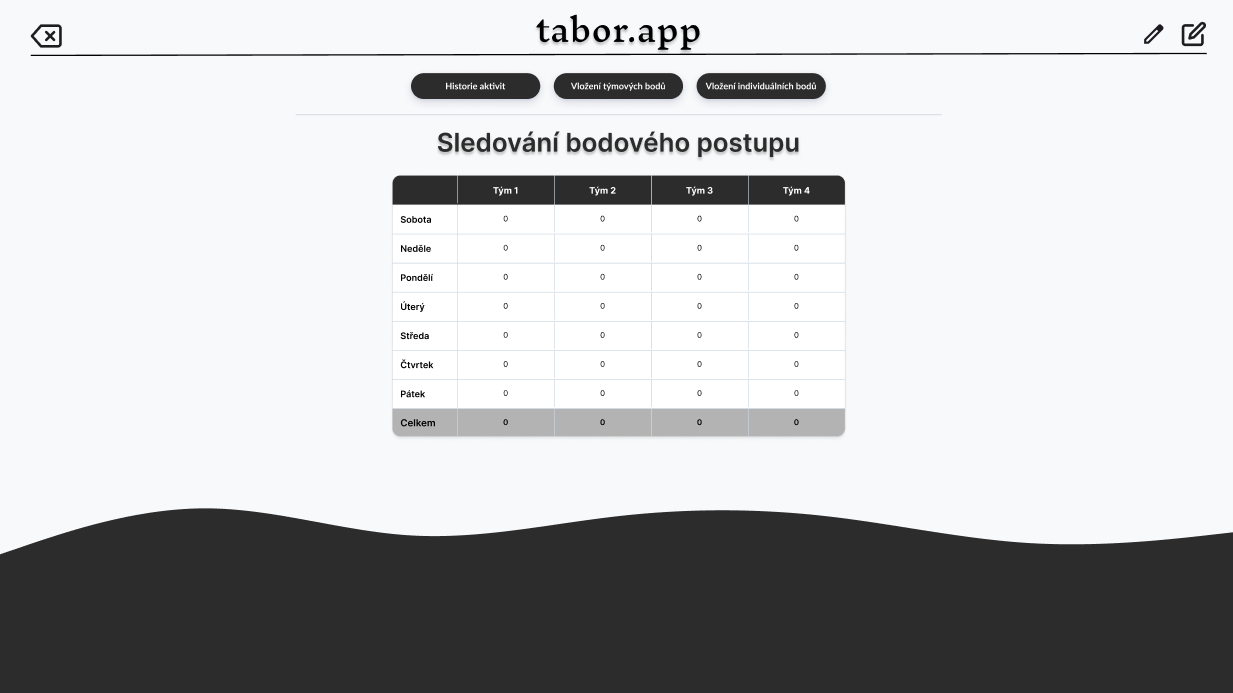
\includegraphics[width=0.8\textwidth]{./pictures/picture1.png}
    \caption{Sledování bodového postupu}
\end{figure}

\textbf{Výběr nebo vytvoření tábora}: Uživatel má možnost buď vybrat již dříve vytvořený 
tábor ze seznamu uložených táborů, čímž se načtou všechny příslušné informace 
(týmy, body, hry), nebo zvolit možnost vytvoření nového tábora. V případě vytvoření nového 
tábora se zobrazí formulář pro zadání základních informací o táboře, jako je název a počet 
týmů.
\begin{figure}[h!]
    \centering
    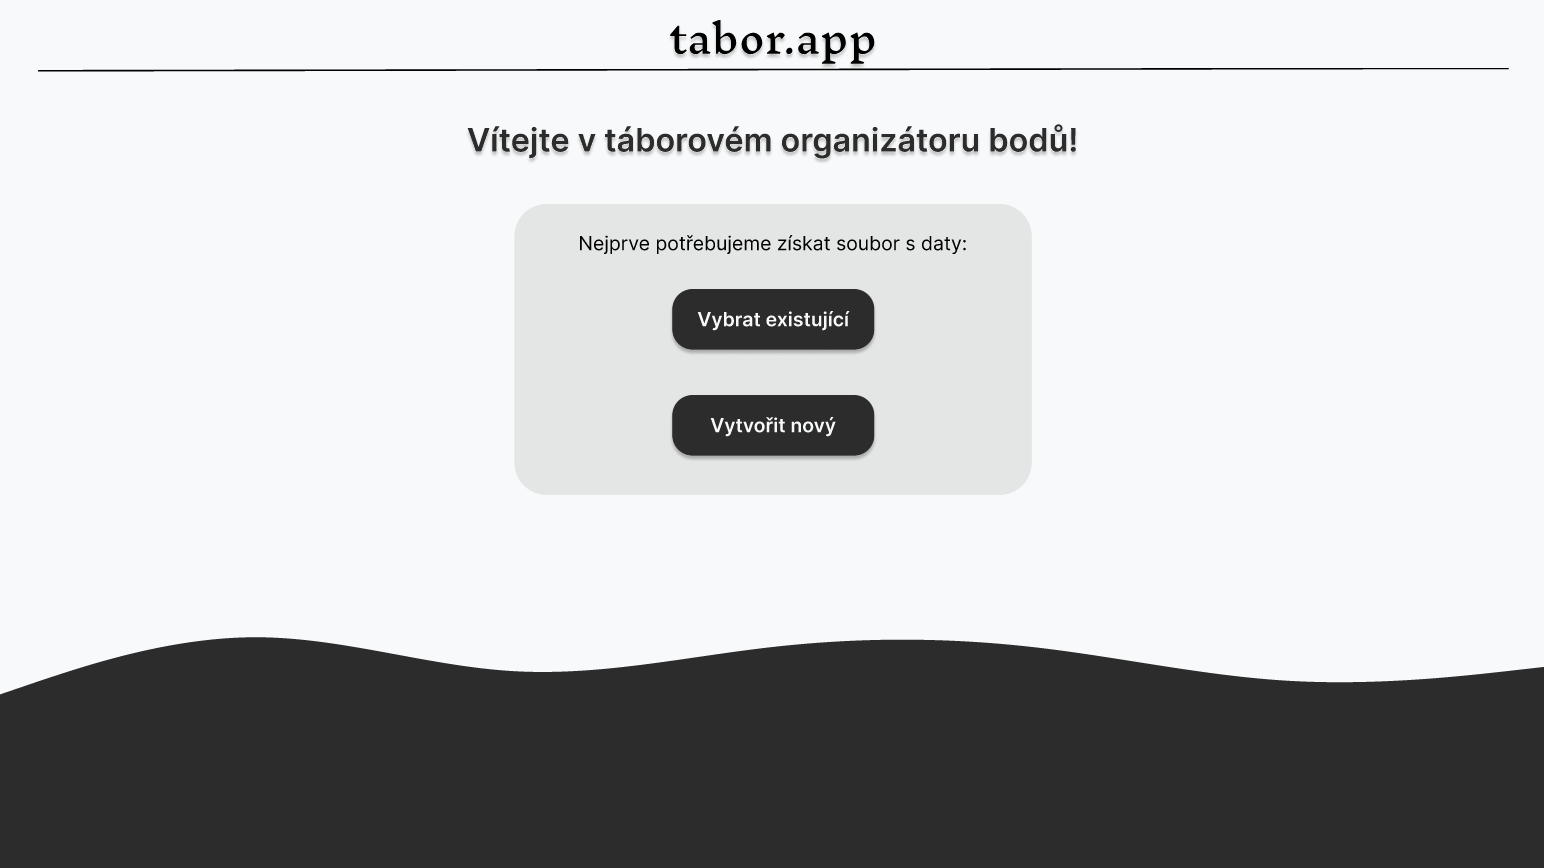
\includegraphics[width=0.8\textwidth]{./pictures/picture8.png}
    \caption{Výběr existujícího tábora nebo vytvoření nového}
\end{figure}

\newpage

\textbf{Vytváření týmů}: Tato část zobrazuje proces tvorby týmů při začátku tábora. 
Uživatel má možnost zadat název týmu, přiřadit týmovou barvu a přidat vedoucí a členy týmu. 
Tato obrazovka je navržena tak, aby byla uživatelsky přívětivá a umožnila rychlé nastavení týmů.
\begin{figure}[h!]
    \centering
    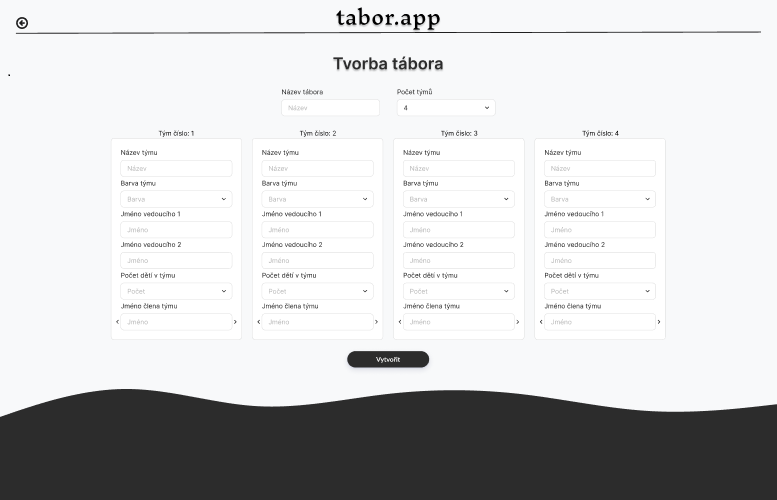
\includegraphics[width=0.8\textwidth]{./pictures/picture2.png}
    \caption{Vytváření týmů}
\end{figure}

\textbf{Zadávání informací o táborových hrách}: Tento screenshot znázorňuje obrazovku pro 
zadávání informací o odehrané hře, jako je typ hry, pořadí týmů a bodové výsledky. Po zadání 
těchto informací se automaticky aktualizují výsledky týmů.
\begin{figure}[h!]
    \centering
    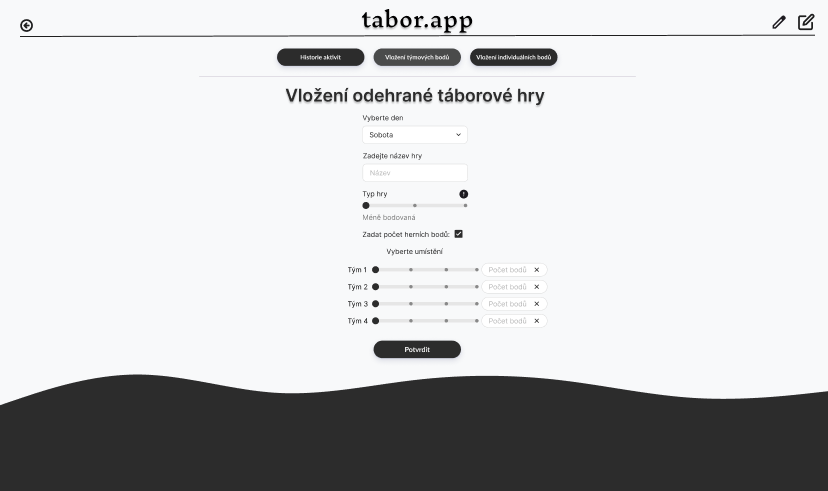
\includegraphics[width=0.8\textwidth]{./pictures/picture3.png}
    \caption{Zadávání informací o táborové hře}
\end{figure}

\newpage

\textbf{Zadání individuálních bodů}: Tento obrázek ukazuje formulář pro zadání 
individuálních bodů pro jednotlivé děti. Uživatel zvolí den, typ aktivity, důvod udělení 
bodů a počet dětí, které body obdrží. Dále je zde seznam dětí, kterým budou body 
přiděleny. Po zadání těchto informací aplikace automaticky aktualizuje statistiky a 
započítá bonusové body do celkového hodnocení.
\begin{figure}[h!]
    \centering
    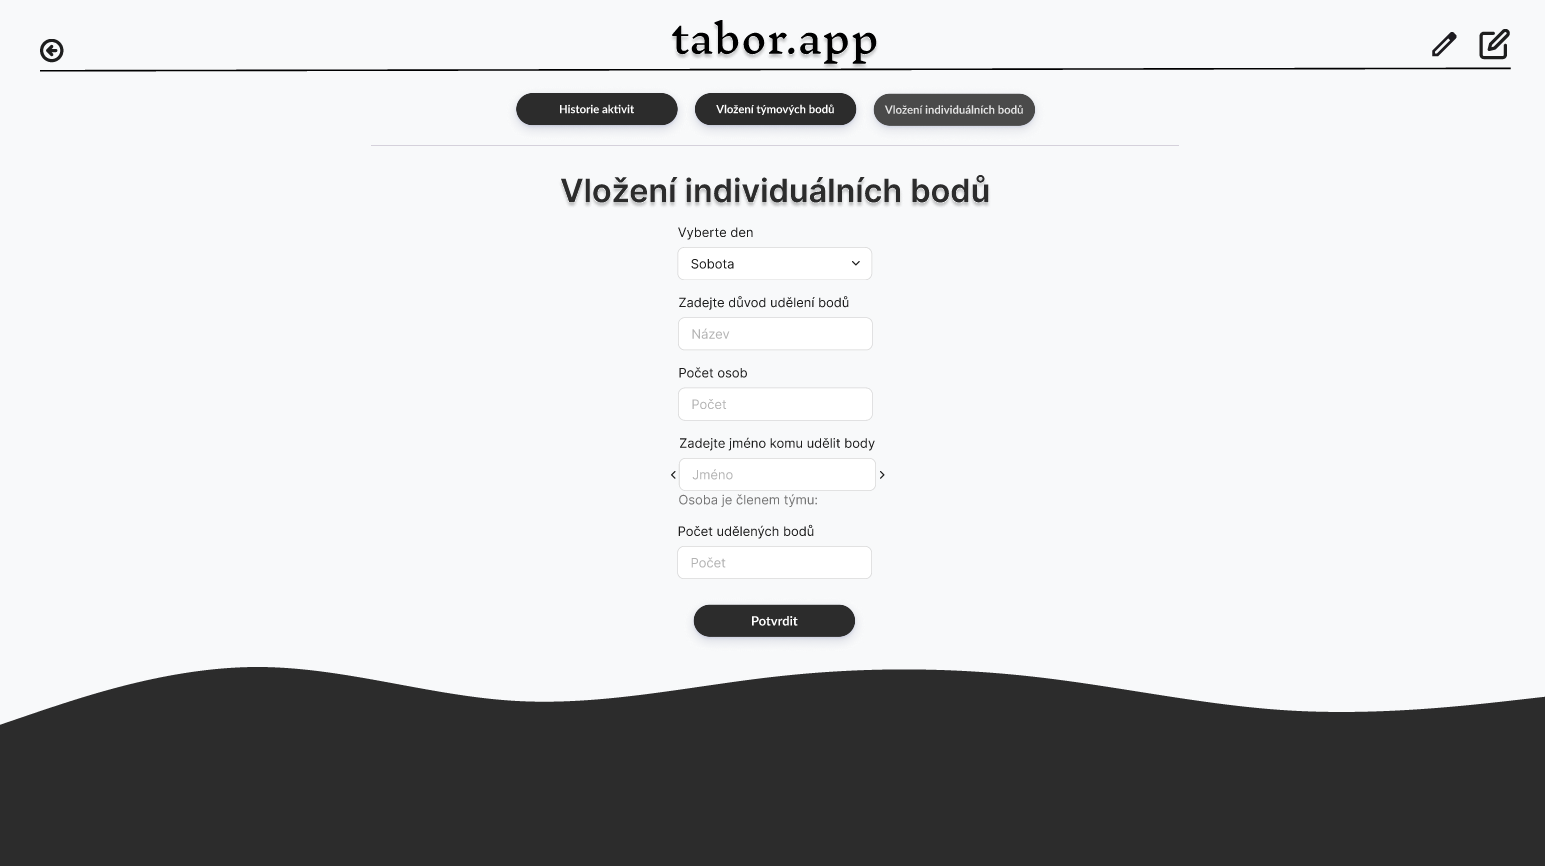
\includegraphics[width=0.8\textwidth]{./pictures/picture6.png}
    \caption{Zadávání individuálních bodů}
\end{figure}

\textbf{Historie aktivit}: Tato obrazovka ukazuje zobrazení historie aktivit, kde uživatel 
zadá konkrétní den a vybere, zda chce vidět týmové nebo individuální aktivity. Zobrazí se 
seznam odehraných her/aktivit, které je možné dále upravit nebo smazat.
\begin{figure}[h!]
    \centering
    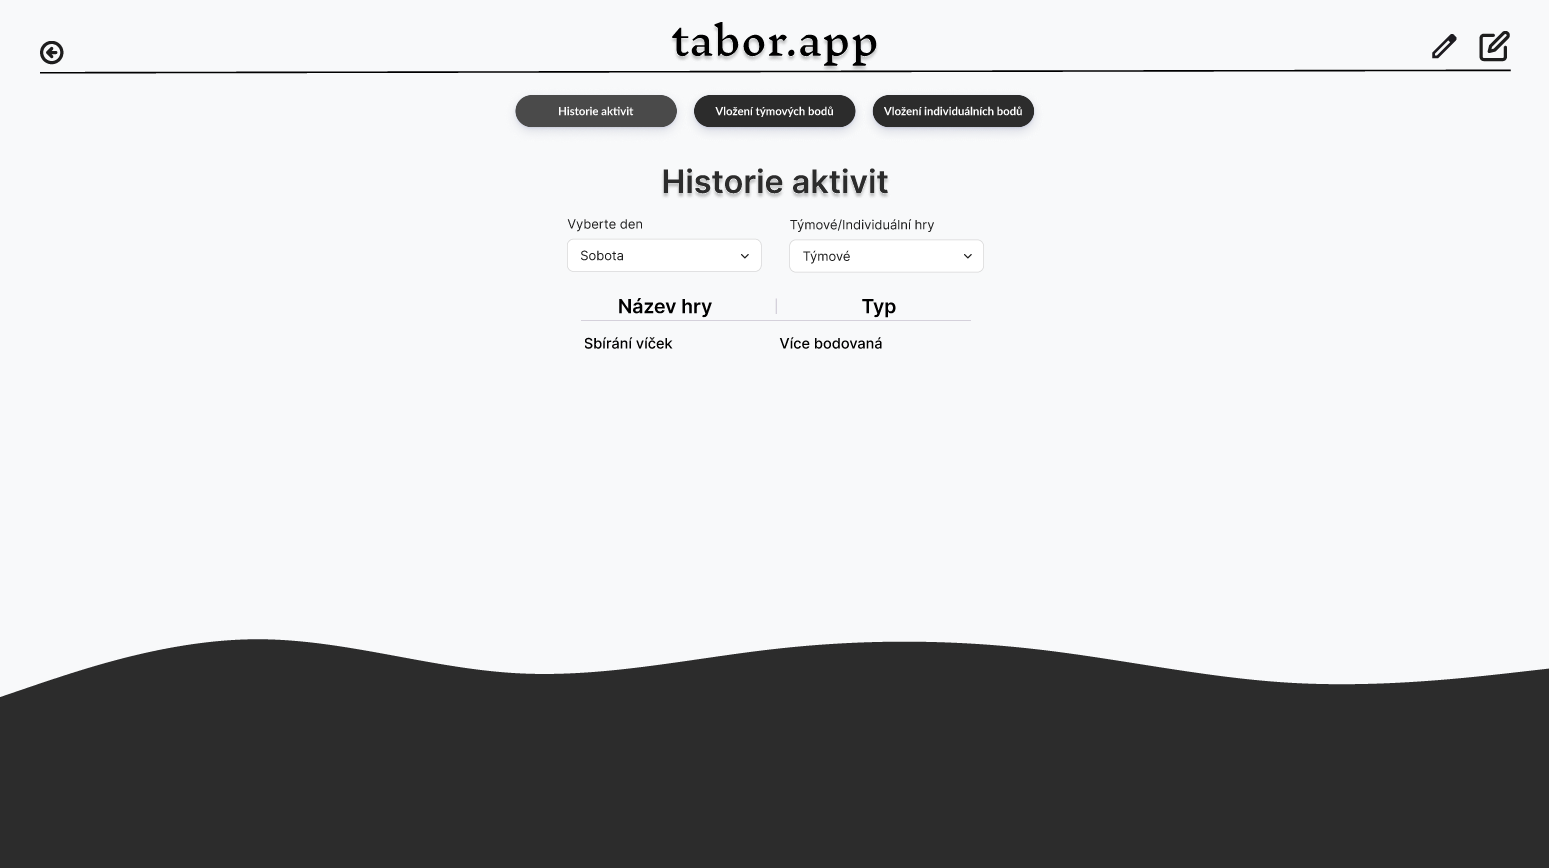
\includegraphics[width=0.8\textwidth]{./pictures/picture4.png}
    \caption{Historie aktivit}
\end{figure}

\newpage

\textbf{Detail hry}: Tento screenshot ukazuje, jak bude vypadat detail rozkliknuté hry. 
Po kliknutí na konkrétní hru se otevře vyskakovací okno s podrobnostmi o hře, které je možné 
editovat nebo smazat.
\begin{figure}[h!]
    \centering
    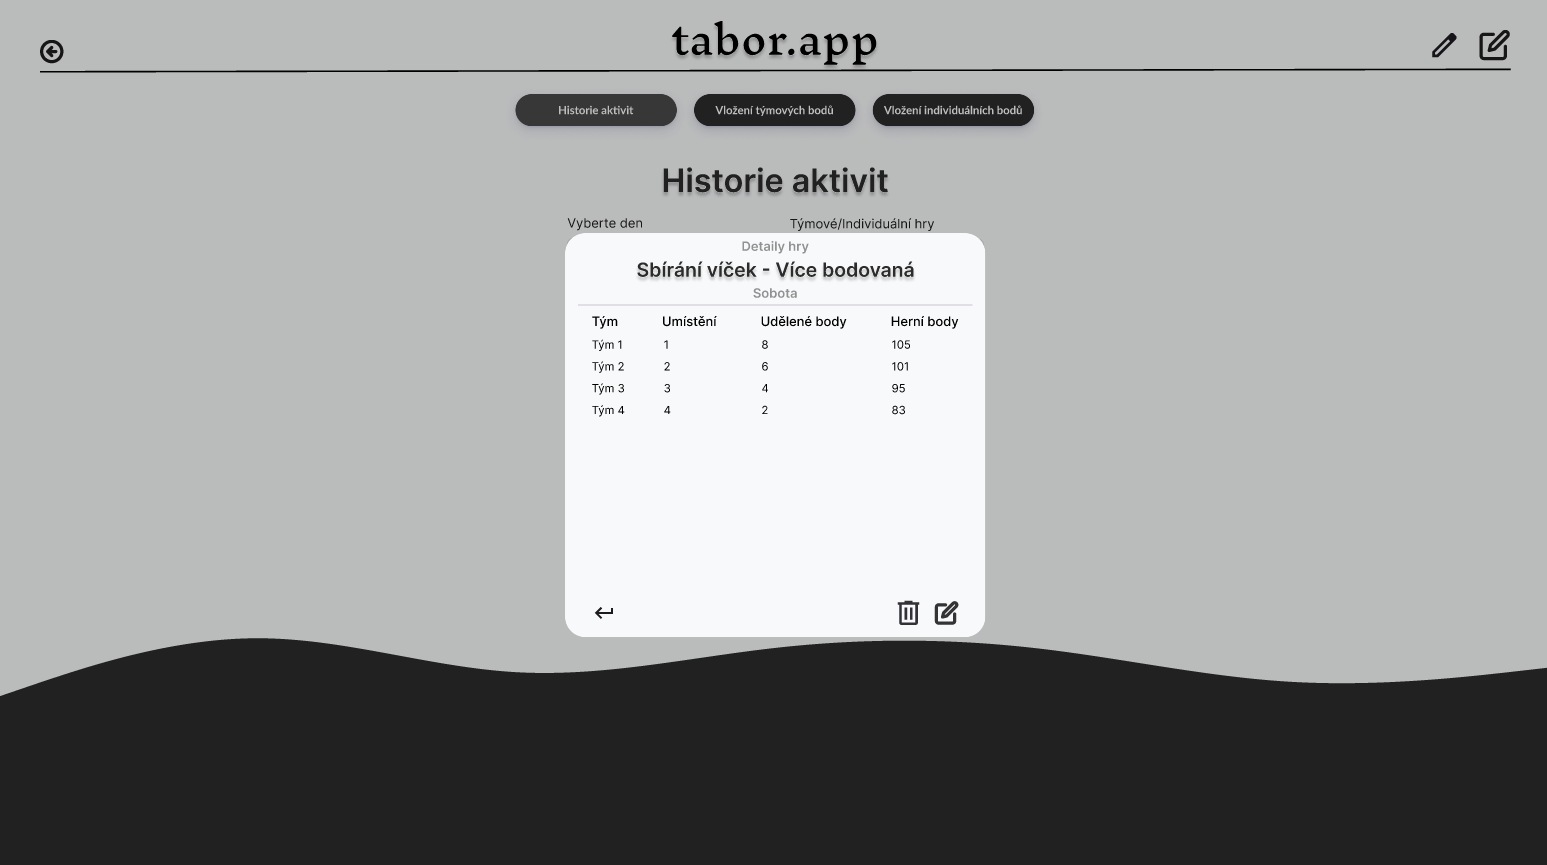
\includegraphics[width=0.8\textwidth]{./pictures/picture5.png}
    \caption{Detail hry}
\end{figure}

\textbf{Úprava bodování her}: Tato obrazovka zobrazuje možnost upravit bodové hodnocení 
pro jednotlivé hry. Uživatel si může vybrat typ hry (méně bodovaná, více bodovaná, 
velmi bodovaná) a přiřadit konkrétní bodové hodnoty pro umístění jednotlivých týmů v dané hře. 
\begin{figure}[h!]
    \centering
    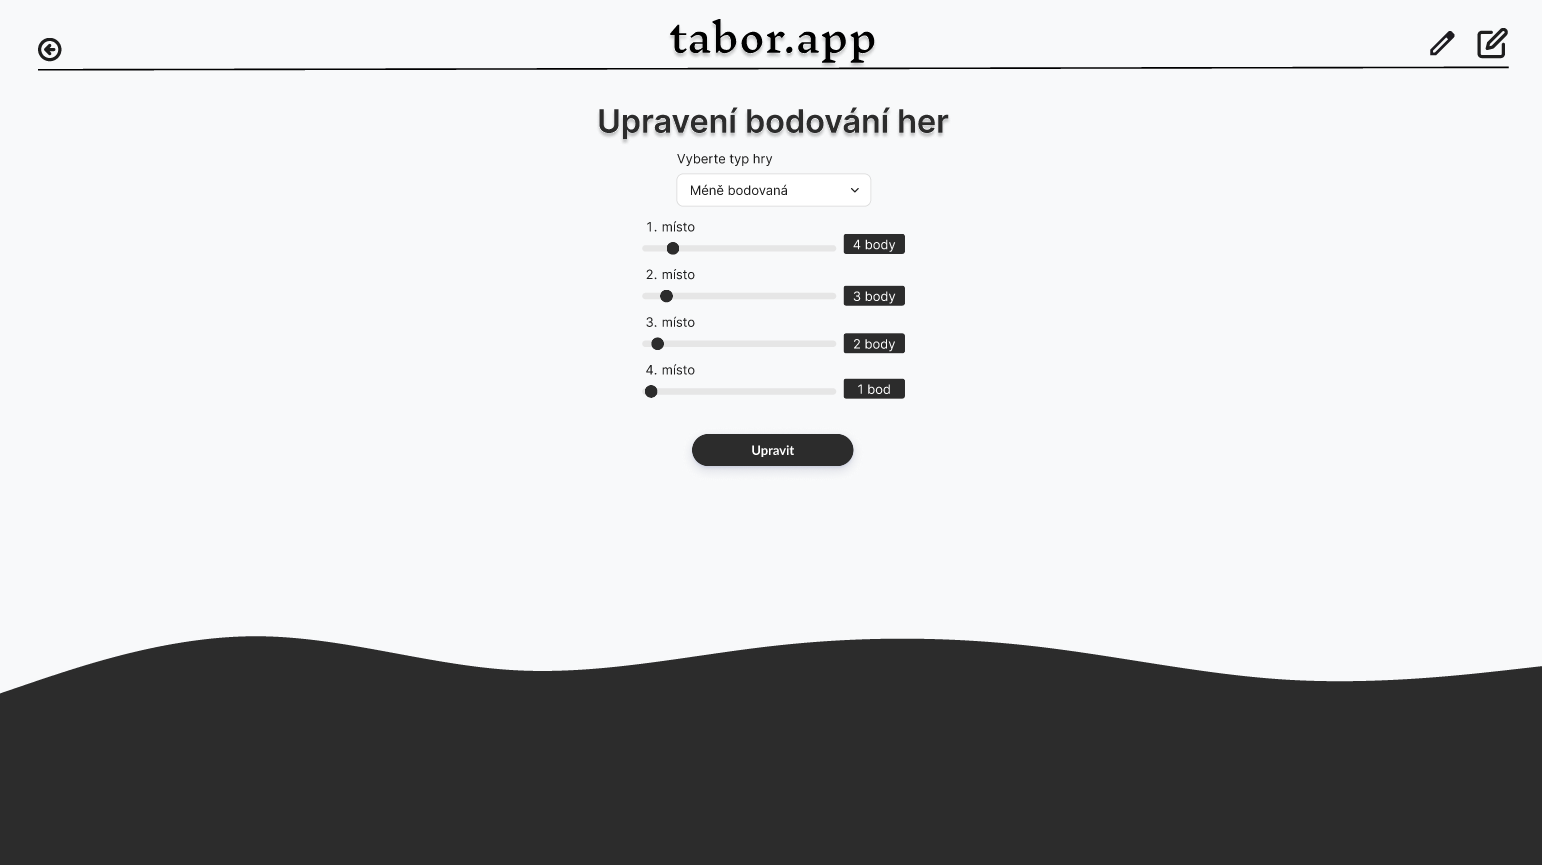
\includegraphics[width=0.8\textwidth]{./pictures/picture7.png}
    \caption{Úprava bodování her}
\end{figure}

\subsection{Výběr technologií}
Tento výběr technologií je založen na jejich jednoduchosti, flexibilitě a schopnosti 
rychle reagovat na měnící se požadavky aplikace.

\subsubsection{Frontend}
Pro tvorbu uživatelského rozhraní jsme zvolili \textbf{React}, populární knihovnu pro 
tvorbu interaktivních a dynamických uživatelských rozhraní. React umožňuje efektivní správu 
komponent, což usnadňuje organizaci a údržbu aplikace. Jeho schopnost rychlého vykreslování 
komponent a asynchronního zpracování dat je klíčová pro plynulou komunikaci s backendem, 
zejména při načítání a ukládání informací o týmech a jejich aktivitách. React také podporuje 
práci s formuláři, což je důležité pro uživatelskou interakci při zadávání bodování a správě 
týmů.

\subsubsection{Backend}
Pro backendovou část aplikace jsme vybrali \textbf{Flask}, minimalistický webový framework pro 
Python. Flask je lehký a flexibilní, což nám umožňuje rychle vyvinout API pro komunikaci s 
frontendem. Data budou uložena ve formátu \textbf{JSON}, což umožňuje jednoduchou manipulaci 
s daty a eliminuje potřebu složitější databáze, přičemž to stačí pro naše požadavky na 
ukládání informací o týmech, hrách a výsledcích.

\subsection{Návrh API pro backend}
Návrh API našeho backendu poskytne klíčové funkce pro správu táboru, týmů, her a aktivit, 
čímž umožní efektivní komunikaci mezi frontendem a backendem. Tento návrh je flexibilní a 
může se v budoucnu měnit podle potřeb vývoje aplikace. Hlavní funkcionality API budou zahrnovat: \\

\textbf{Správa táboru:}
Funkce pro:
\begin{itemize}
    \item Získání seznamu táborů.
    \item Vytváření nových táborů.
    \item Aktualizaci detailů tábora.
\end{itemize}

\textbf{Správa týmů:}
Funkce pro:
\begin{itemize}
    \item Získání seznamu týmů.
    \item Přidávání nových týmů.
    \item Aktualizaci informací o týmech (jméno, barva, členové).
\end{itemize}

\textbf{Správa her a aktivit:}
Funkce pro:
\begin{itemize}
    \item Přidávání her a aktivit.
    \item Záznam výsledků her a aktivit.
    \item Udělování bonusových bodů účastníkům nebo týmům.
\end{itemize}

\subsection{Klíčové datové struktury}
V návrhu aplikace jsme definovali několik klíčových datových struktur, které slouží k 
uchovávání a správě dat v systému:

\begin{itemize}
    \item \textbf{Tábor}: Hlavní entita, která obsahuje název tábora a seznam týmů.
    \item \textbf{Tým}: Uchovává název týmu, jeho barvu, seznam vedoucích a členů, a celkový 
    počet bodů.
    \item \textbf{Týmová hra}: Obsahuje informace o odehrané hře, včetně data, typu hry, 
    pořadí týmů a bodových výsledků.
    \item \textbf{Individuální aktivita}: Uchovává informace o bonusových bodech, včetně data, 
    důvodu, počtu dětí a jejich seznamu.
    \item \textbf{Typ hry}: Určuje bodové hodnoty přiřazené různým typům her 
    (např. méně bodovaná, více bodovaná, velmi bodovaná) a body za umístění v konkrétní hře.
\end{itemize}

\subsection{Napojení FE na BE}
Frontend bude komunikovat s backendem prostřednictvím HTTP požadavků (GET, POST, PUT, DELETE). 
Při interakci s uživatelem frontend odešle data na backend, který je zpracuje a vrátí 
odpověď pro aktualizaci uživatelského rozhraní. Tento proces umožní dynamickou interakci 
mezi frontendem a backendem. V současnosti je funkcionalita naší aplikace omezená, nejsme 
si ještě úplně jisti všemi detaily, a proto je možné, že se některé prvky v budoucnu změní.

\section{Závěr}

Tento projekt představuje naši první zkušenost s vývojem webové aplikace a tvorby 
uživatelského rozhrání. I když jsme se snažili vytvořit co nejefektivnější řešení pro správu 
táborových her a bodování, jsme stále začátečníci a jsme si vědomi toho, že aplikace může 
vyžadovat další vylepšení.

\end{document}